%-*- Mode:LaTeX; -*-      
\documentclass[11pt]{article}
\usepackage{vmargin}		% Force narrower margins
\setpapersize{USletter}
\setmarginsrb{1.0in}{1.0in}{1.0in}{0.6in}{0pt}{0pt}{0pt}{0.4in}
\setlength{\parskip}{.1in}  % removed space between paragraphs
\setlength{\parindent}{0in}

\usepackage{epsfig}
\usepackage{graphicx}

\begin{document}

\large
\begin{center}
{\bf CS-5340/6340, Written Assignment \#2} \\
{\bf DUE: Wednesday, Sept. 30, 2015 by 11:00pm}
\end{center}
\normalsize

\begin{enumerate}  

\item (24 pts) For each recursive transition network (RTN) below,
  write a grammar that accepts exactly the same language as the
  RTN. \\ 
  


\hrule
(a) RTN \#1: 
\begin{center}
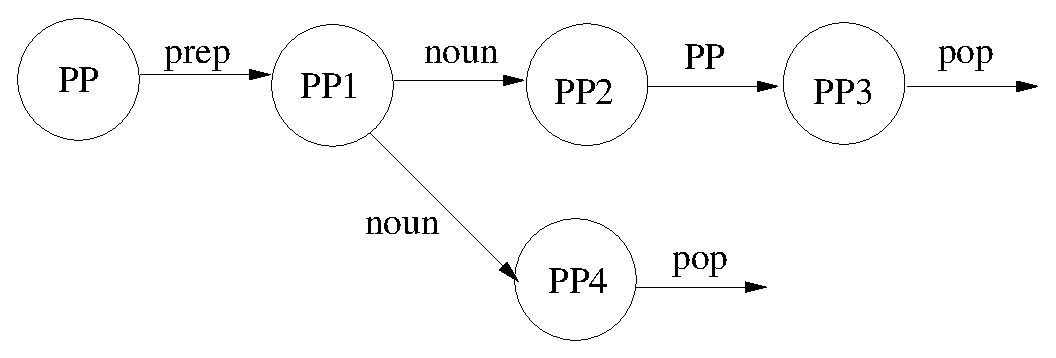
\epsfig{file=rtn3.eps,height=1.5in}
\end{center}

  PP $\rightarrow$ prep noun PP \\
  PP $\rightarrow$ prep noun\\
	
\hrule 
(b) RTN \#2: 
\begin{center}
~ 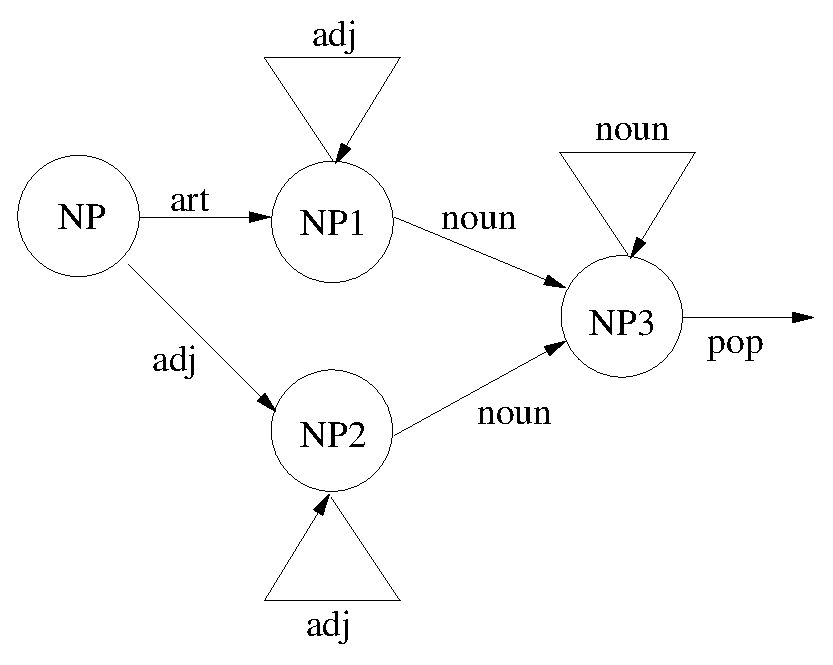
\epsfig{file=rtn1.eps,height=2.5in}
\end{center}

NP $\rightarrow$  art NP1\\
NP $\rightarrow$  adj NP2\\
NP1 $\rightarrow$  adj NP1\\
NP2  $\rightarrow$  adj NP2 \\
NP1 $\rightarrow$ NP3\\
NP2 $\rightarrow$ NP3\\
NP3 $\rightarrow$ noun NP3\\
NP3 $\rightarrow$  noun\\

If we were to write it more generically like the example which Professor worked out in class, it would be 

NP $\rightarrow$  art X\\
NP $\rightarrow$  adj X\\
X $\rightarrow$  adj X\\
X $\rightarrow$ Y\\
Y $\rightarrow$ noun Y\\
Y $\rightarrow$  noun\\


\hrule
(c) RTN \#3: 
\begin{center}
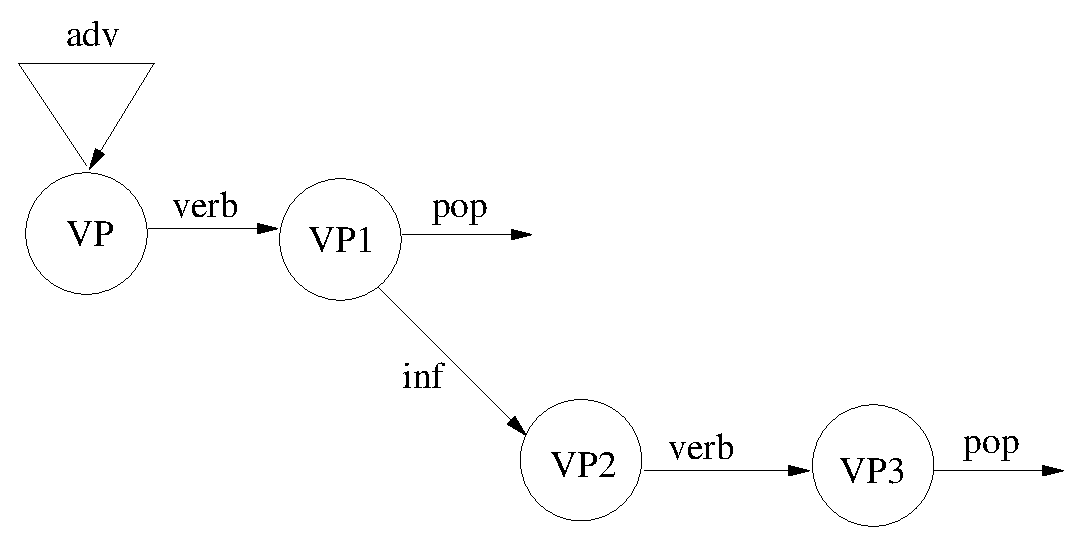
\epsfig{file=rtn2.eps,height=2in}
\end{center}

VP $\rightarrow$ adv VP\\
VP $\rightarrow$  verb inf verb\\
VP $\rightarrow$  verb\\

\hrule
%% ===============================================================
% QUESTION #2 : Bottom-up Chart Parsing
%% ===============================================================

\item (30 pts) Consider the grammar and lexicon below:

\begin{center}
\begin{tabular}{|ll|} \hline
\textbf{Grammar} & \textbf{Lexicon} \\  \hline
S $\rightarrow$ NP VP & {\it trust} : noun, verb \\
NP $\rightarrow$ noun & {\it shrinks} :  noun, verb \\
NP $\rightarrow$ noun noun  & ~ \\
VP $\rightarrow$ verb & ~ \\
VP $\rightarrow$ verb NP & ~ \\  \hline
\end{tabular}
\end{center}

\vspace*{.1in} List all of the entries that would be put on the chart during
{\bf bottom-up chart parsing} for the sentence {\bf `trust shrinks'}.
Each chart entry should be a constituent or a rule, with a start
and end position indicating which words have been matched by the
constituent or rule.

To get you started, the list below contains chart entries for the
part-of-speech tag constituents for the words `trust' and `shrinks'
and for two rules that should be on the chart. Your job is to complete
this list by adding the rest of the constituents and rules that would
be put on the chart during parsing.

For the rules, please use an asterisk (*) to separate the components
of the rule that have been matched from the ones that have not yet been
matched. For example, the rule ``NP $\rightarrow$ noun * noun [1-2]'' means that
 the first noun in this rule has been successfully matched with a
 constituent starting in position 1 and ending in position 2. \\




\begin{center}
{\bf Complete the Chart Entries for Bottom-up Chart Parsing of `Trust Shrinks'} 
\end{center}

\begin{center}
\begin{tabular}{lc} 
{\bf Constituent/Rule~~~} & {\bf ~~~Start-End} \\ \hline
noun(``trust'') &  [1-2] \\
verb(``trust'') & [1-2] \\
noun(``shrinks'') & [2-3] \\
verb(``shrinks'') & [2-3] \\
NP $\rightarrow$ noun * & [1-2] \\
NP  & [1-2]\\
NP $\rightarrow$ noun * noun & [1-2] \\ 
VP $\rightarrow$ verb * & [1-2] \\ 
VP & [1-2]\\
VP $\rightarrow$ verb * NP &[1-2]\\
S $\rightarrow$ NP *VP & [1-2]\\
NP $\rightarrow$ noun * & [2-3]\\
NP  & [2-3] \\
NP $\rightarrow$ noun noun * (carried over rule gets completed here) & [1-3] \\ 
NP & [1-3]\\
NP $\rightarrow$ noun * noun & [2-3] \\ 
VP $\rightarrow$ verb NP *(carried over rule gets completed here) &[1-3]\\
VP & [1-3]\\
VP $\rightarrow$ verb * & [2-3]\\
VP & [2-3]\\
VP $\rightarrow$ verb * NP & [2-3]\\
S $\rightarrow$ NP VP * & [1-3] \\
S & [1-3] \\\hline

%{\it  ... add remaining entries here ...} \\
\end{tabular}
\end{center}


%% ===============================================================
% QUESTION #3 : basic probs / n-grams
%% =============================================================

\item (16 pts) Consider the following tongue twister: 

\begin{quote}
{\tt whether the weather is warm , whether the weather is hot , we have to
put up with the weather , whether we like it or not .}
\end{quote}

Using the tongue twister above as your text corpus, compute the
following probabilities. Note that this text sample contains 28 words
because each comma  and period counts as a word. {\it Please leave
  your answers in fractional form with 
  the frequency counts used for the computation! For   example, we
  want to see answers of the form 14/28, not .50}  

\begin{itemize}

\item P(``or'')  = $\frac{1}{28}$\\

\item P(``weather'') = $\frac{3}{28}$\ \\

\item P(``weather'' $\mid$ ``the'') = $\frac{3}{3}$ =1\ \\

\item P(``whether'' $\mid$ ``we'')  = $\frac{0}{2}$ = 0\\

\item P(``warm'' $\mid$ ``is'') =$\frac{1}{2}$ \\

\item P(``hot'' $\mid$ ``weather'', ``is'') =$\frac{1}{2}$  \\

\item P(``is'' $\mid$ ``the'', ``weather'') = $\frac{2}{3}$  \\

\item P(``up'' $\mid$ ``to'', ``put'') = $\frac{1}{1}$ = 1 \\


\end{itemize}


%% ===============================================================
% QUESTION #4 :  recall, precision, F scores
%% =============================================================


\item (18 pts) Consider the sentence:  \\
{\tt John Smith planned to fish for silver trout and char but he forgot to bring the fishing gear}

Suppose your part-of-speech (POS) tagger assigns these POS tags to the sentence:

{\tt John/NOUN Smith/NOUN planned/VERB to/PREP fish/NOUN for/PREP silver/NOUN trout/NOUN
and/CONJ char/VERB but/CONJ he/PRO forgot/VERB to/INF bring/VERB the/ART fishing/VERB gear/NOUN}

Assume that the {\bf correct} POS tags for the sentence are:

{\tt John/NOUN Smith/NOUN planned/VERB to/INF fish/VERB for/PREP silver/ADJ
trout/NOUN and/CONJ char/NOUN but/CONJ he/PRO forgot/VERB to/INF
bring/VERB the/ART fishing/GER gear/NOUN} \\

Based on the information above, answer the questions below. Please
leave your answers in fractional form!

\begin{enumerate}

\item What is the overall accuracy of your POS tagger?\\
$\frac{13}{18}$ 


\item What is the recall of your POS tagger for verbs?\\
$\frac{3}{4}$ 

\item What is the precision of your POS tagger for verbs?\\
$\frac{3}{5}$ 

\item What is the recall of your POS tagger for nouns?\\
$\frac{4}{5}$ 

\item What is the precision of your POS tagger for nouns?\\
$\frac{4}{6}$ 

\item What is the recall of your POS tagger for prepositions (PREP tag)? \\
$\frac{1}{1}$ 

\item What is the precision of your POS tagger for prepositions (PREP tag)?\\
$\frac{1}{2}$ 

\item Using the \textbf{correct} POS tags, what is the lexical
  generation probability P(planned $\mid$ VERB)?\\
$\frac{1}{4}$ 
\item Using the \textbf{correct} POS tags, what is P(VERB $\mid$
  planned), which means the probability that the word ``planned''
  should have the tag VERB?\\
  $\frac{1}{1}$ 

\end{enumerate}


\newpage
%% ===============================================================
% QUESTION #5 :  N-gram language modeling for POS tagging
%% =============================================================

\item (12 pts) Consider the   probability that the sentence {\it ``A
    witty saying proves nothing''} 
  (a quote from Voltaire) should be assigned the 
  part-of-speech (POS) tag sequence {\it ``ART ADJ NOUN VERB NOUN''}. 

\begin{center}
{\it P(ART ADJ NOUN VERB NOUN $\mid$ A witty saying proves nothing)}
\end{center}

If you perform statistical part-of-speech tagging with N-gram language
models to compute  this probability, show the equation that would
be used for each type of N-gram language model below. 
You must instantiate the equation with the specific words and
part-of-speech tags shown above, but no numbers are needed. 

If necessary, use the symbol $\phi_{0}$ to denote the beginning of a
sentence (i.e., the position immediately to the left of the first
word) and the symbol $\phi_{-1}$ to denote two positions to the left
of the first word.

\begin{enumerate}
\item Show the equation using a unigram language model. \\
=$\prod\limits_{i=1}^{n} P(T_i) * P(w_i |T_i)$\\

=[P(A$|$ART) * P(ART)]*  [P(witty$|$ADJ) * P(ADJ)] * [P(saying$|$NOUN) * P(NOUN)] * [P(proves$|$VERB) * P(VERB)] * [P(nothing$|$NOUN) * P(NOUN)] \\

\item Show the equation using a bigram language model. \\ 

=$\prod\limits_{i=1}^{n} P(T_i | T_{i-1}) * P(w_i |T_i)$\\
= [P(ART $|$ $\phi$ ) * P(A$|$ART) ] * [ P(ADJ$|$ART) * P(witty$|$ADJ) ] * [P(NOUN$|$ADJ) * P(saying$|$NOUN)] *
[P(VERB$|$NOUN) * P(proves$|$VERB)] * [P(NOUN$|$VERB) * P(nothing$|$NOUN)] \\

\item Show the equation using a trigram language model.
Each trigram should be written as $P(Z \mid X~Y)$, where X
precedes Y in the input. \\

=$\prod\limits_{i=1}^{n} P(T_i | T_{i-2},T_{i-1}) * P(w_i |T_i)$\\

=[P(ART $|$ $\phi_{i-1} , \phi_i$) * P(A$|$ART)] * [P(ADJ$|\phi_i$,ART ) * P(witty$|$ADJ)] *[P(NOUN$|$ ART, ADJ) * P(saying$|$NOUN)] * [P(VERB$|$ADJ, NOUN) * P(proves$|$VERB)] * [P(NOUN$|$NOUN, VERB) * P(nothing$|$NOUN)]  
\end{enumerate}

\underline{\textbf{Question \#6 is for CS-6340 students ONLY!}}  \\

%% ================================================================
% QUESTION #5: Top-down Chart Parsing
%% ================================================================

\item (18 pts) Consider the grammar and lexicon below:

\begin{center}
\begin{tabular}{|ll|} \hline
\textbf{Grammar} & \textbf{Lexicon} \\  \hline
S $\rightarrow$ NP VP & {\it trust} : noun, verb \\
NP $\rightarrow$ noun & {\it shrinks} :  noun, verb \\
NP $\rightarrow$ noun noun  & ~ \\
VP $\rightarrow$ verb & ~ \\
VP $\rightarrow$ verb NP & ~ \\  \hline
\end{tabular}
\end{center}

\vspace*{.1in} List all of the entries that would be put on the chart during
{\bf top-down chart parsing} for the sentence {\bf `trust shrinks'}.
Each chart entry should be a constituent or a rule, with a start
and end position indicating which words have been matched by the
constituent or rule.

To get you started, the list below contains chart entries for the
part-of-speech tag constituents for the words `trust' and `shrinks'
and for three rules that should be on the chart. Your job is to complete
this list by adding the rest of the constituents and rules that would
be put on the chart during parsing.

For the rules, please use an asterisk (*) to separate the components
of the rule that have been matched from the ones that have not yet been
matched. For example, the rule ``NP $\rightarrow$ * noun noun [1-1]'' means that
no nouns in this rule have been matched yet but the rule
can begin matching constituents starting in position 1. \\ 

\begin{center}
{\bf Complete the Chart Entries for Top-down Chart Parsing of `Trust Shrinks'} 
\end{center}

\begin{center}
\begin{tabular}{lc} 
{\bf Constituent/Rule~~~} & {\bf ~~~Start-End} \\ \hline
noun(``trust'') &  [1-2] \\
verb(``trust'') & [1-2] \\
noun(``shrinks'') & [2-3] \\
verb(``shrinks'') & [2-3] \\
S $\rightarrow$ * NP VP & [1-1] \\
NP $\rightarrow$ * noun & [1-1] \\ 
NP $\rightarrow$ * noun noun & [1-1] \\ 
NP $\rightarrow$  noun * & [1-2] \\ 
NP & [1-2]\\
NP $\rightarrow$  noun * noun & [1-2] \\ 
S $\rightarrow$  NP * VP & [1-2] \\
VP $\rightarrow$ * verb  &[2-2]\\
VP $\rightarrow$ * verb  NP & [2-2]\\
VP $\rightarrow$  verb * &[2-3]\\
VP & [2-3]\\
VP $\rightarrow$  verb *  NP &[2-3]\\
S $\rightarrow$  NP  VP * & [1-3] \\
S & [1-3]\\\hline

\end{tabular}
\end{center}



\end{enumerate}  % END OF WRITTEN QUESTIONS

\end{document}
